\documentclass[12pt]{article}
\usepackage[margin=1in]{geometry}
\usepackage[all]{xy}

\usepackage{amsmath,amsthm,amssymb,color,latexsym,soul}
\usepackage{geometry}        
\geometry{letterpaper}    
\usepackage{graphicx}
\usepackage{enumitem}
\usepackage{listings}
\usepackage{xcolor}
\usepackage{bm}
\usepackage{hyperref}
\hypersetup{
    colorlinks=true,
    linkcolor=blue,
    filecolor=magenta,      
    urlcolor=cyan,
    citecolor=blue,
}

\definecolor{codegreen}{rgb}{0,0.6,0}
\definecolor{codegray}{rgb}{0.5,0.5,0.5}
\definecolor{codepurple}{rgb}{0.58,0,0.82}
\definecolor{backcolour}{rgb}{0.95,0.95,0.92}

\lstdefinestyle{mystyle}{ % taken from: https://www.overleaf.com/learn/latex/Code_listing
    backgroundcolor=\color{backcolour},   
    commentstyle=\color{codegreen},
    keywordstyle=\color{magenta},
    numberstyle=\tiny\color{codegray},
    stringstyle=\color{codepurple},
    basicstyle=\ttfamily\footnotesize,
    % breakatwhitespace=false,         
    breaklines=true,                 
    captionpos=b,                    
    keepspaces=true,                 
    % numbers=left,                    
    numbersep=5pt,                  
    % showspaces=false,                
    % showstringspaces=false,
    % showtabs=false,                  
    % tabsize=2
}

\lstset{style=mystyle}

\newtheorem{task}{Task}
\newenvironment{solution}[1][\it{Solution}]{\textbf{#1. } }{$\square$}
\newtheorem{subtask}{\; \; \it{Part}}


\begin{document}
\noindent Asaad Mohammedsaleh \hfill CS249 Assignment 2\\
KAUST Spring 2025 \hfill Genome Assembly and Evaluation


\hrulefill

\section{Introduction}

In this assignment, I had the opportunity to work with assembling and evaluating genome assemblies. 

In the first part of the assignment, I implemented the De Bruijn Graph (DBG) and Overlap-Layout-Consensus (OLC) algorithms.
The assignment sheet provided a toy dataset to test the algorithms and a larger more realistic dataset of Middle East respiratory
syndrome-related coronavirus (MERS-CoV) genome. I evaluated the performance of these algorithms on the datasets and compared them against each other and against a more established tool, SPAdes.

In the second part of the assignment, I worked with a lizard genome and evaluated the performance of the assembly using the tools described in the assignment sheet. 

The implementation of the algorithms and the evaluation of the performance are described in the following sections. The code is available at \url{https://github.com/Asaad47/BioAlgos-Assignment2}.

\section{Task 1.1 De Bruijn Graph (DBG) Assembly}

Requirements of this algorithm are:
\begin{itemize}
    \item Takes FASTQ files as input
    \item Constructs a de Bruijn graph from k-mers (with user-defined k)
    \item Identifies contigs by finding Eulerian paths
    \item Outputs contigs as a FASTA file
\end{itemize}

The implementation of the algorithm can be found in \texttt{src/dbg.go} file. The main function to handle the algorithm's components is \texttt{DBGAssembler}.
Then, there are two helper functions: \texttt{constructDeBruijnGraph} and \texttt{walkGraph}.

\texttt{constructDeBruijnGraph} constructs the de Bruijn graph from the reads. It first creates a map of k-mers to their nodes. Then, it adds the edges to the graph. The graph is represented as a map of k-mers to their nodes, where each node is a struct with the k-mer string, its outgoing edges (a map of other k-mers to the number of times they appear in the reads), and its incoming edges (a map of other k-mers to the number of times they appear in the reads).

\texttt{walkGraph} looks at nodes with no incoming edges and picks the longest outgoing edge, which would be a greedy approach on the most occurence of the k-mer. It then follows the edge to the next node and repeats the process until it reaches a node with no outgoing edges. It then adds the collected contig from this path to the list of contigs. It repeats this process for all nodes with no incoming edges, so essentially the output has the same number of contigs as the number of nodes with no incoming edges.

\texttt{DBGAssembler} then writes the contigs to a FASTA file.

\section{Task 1.2 Overlap-Layout-Consensus (OLC) Assembly}

Requirements of this algorithm are:
\begin{itemize}
    \item Takes FASTQ files as input
    \item Computes all-vs-all read overlaps and constructs an overlap graph,
    using the minimum overlap length n as a parameter
    \item Identifies non-branching paths in the graph
    \item Generates a layout of reads
    \item Computes a consensus sequence for each contig
    \item Outputs contigs as a FASTA file
\end{itemize}

The implementation of the algorithm can be found in \texttt{src/olc.go} file. The main function to handle the algorithm's components is \texttt{OLCAssembler}. Then, there are three helper functions: \texttt{overlap}, \texttt{layout}, and \texttt{consensus}.

\texttt{overlap} computes all-vs-all read overlaps and constructs an overlap graph, using the minimum overlap length \texttt{min\_overlap} as a parameter. It returns a map of reads to their nodes, where each node is a struct with the read string, its outgoing edges (a map of other reads to the largest overlap size), and its incoming edges (a map of other reads to the largest overlap size).
The implementation is a naive approach that iterates over all pairs of reads and checks for overlaps, which worked sufficiently for the assignment's datasets.

\texttt{layout} reduces the size of the overlap graph by removing 1-hop and 2-hop inferrible edges as described in the lecture notes of Johns Hopkins slides \cite{olc_lecture_notes}. During the process, it updates the overlap graph by combining reads that have single in-edges and single out-edges. It then outputs the list of reads of the updated overlap graph as contigs.

\texttt{consensus} is a greedy algorithm that starts from a read with no incoming edges and follows the longest outgoing edge until it reaches a read with no outgoing edges. It then adds the collected contig from this path to the list of contigs. It repeats this process for all reads with no incoming edges, so essentially the output has the same number of contigs as the number of reads with no incoming edges. This is not an optimal solution, but it happened to be a good approximation for the assignment's datasets.



\section{Task 1.3 Applications of assembly algorithms}

\subsection{Task 1.3.1}

\begin{figure}[h!]
    \centering
    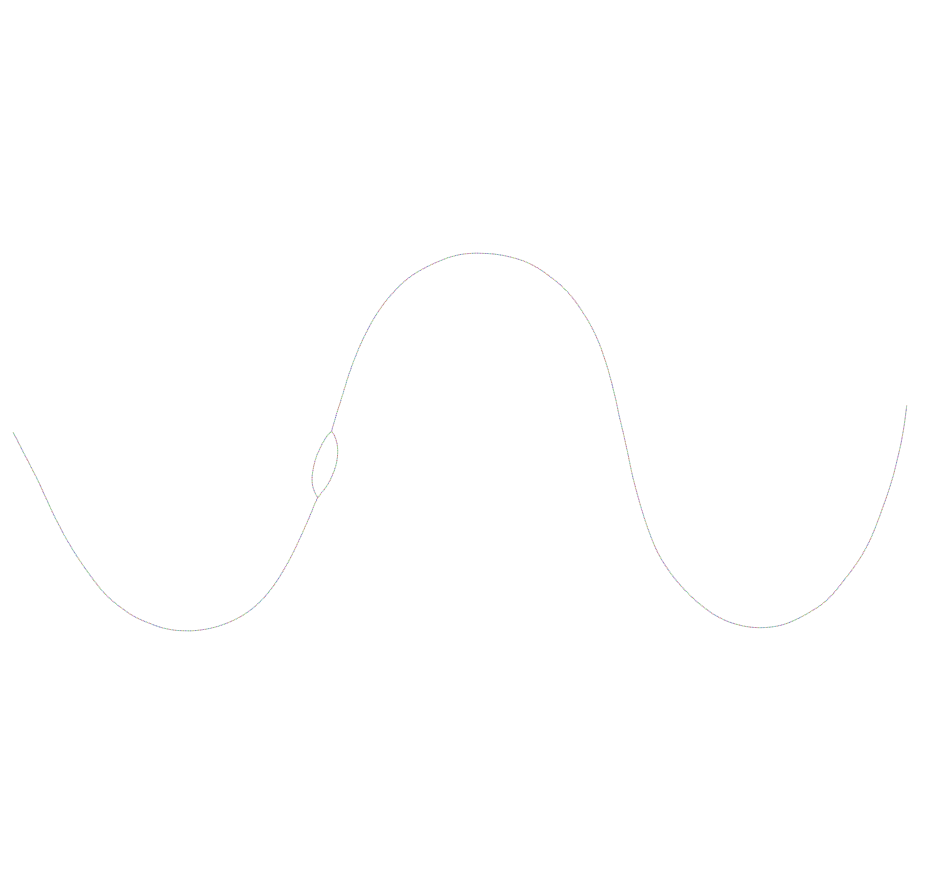
\includegraphics[width=0.5\textwidth]{../toy_dataset/reads_b_k_40.png}
    \caption{Bandage visualization of DBG for $k=40$}
    \label{fig:dbg_k_40}
\end{figure} 

Figure \ref{fig:dbg_k_40} shows the DBG for $k=40$ on reads\_b.fastq visualized using Bandage. A bubble can be seen in the middle of the graph, which suggests that the assembly is not optimal to reconstruct the original genome.
This hints toward using a larger $k$ value to get a better assembly, where in the next section, we will see that using $k=45$ gives a better assembly.

\subsection{Task 1.3.2}

\begin{figure}[h!]
    \centering
    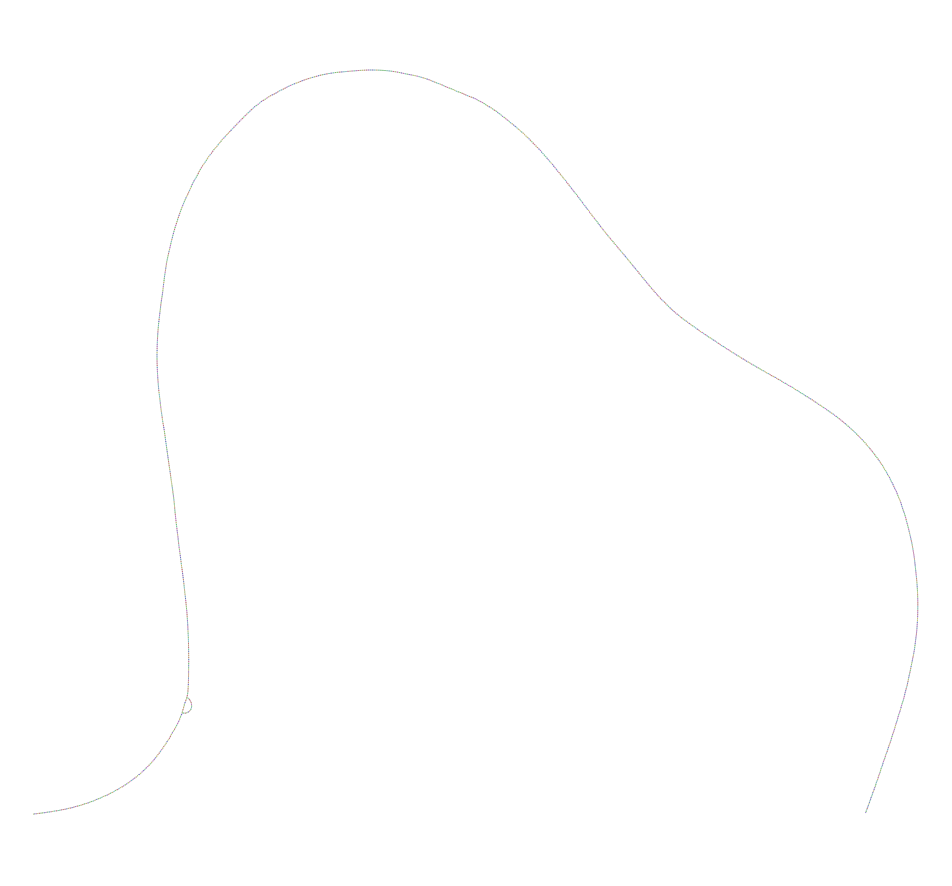
\includegraphics[width=0.5\textwidth]{../toy_dataset/r-k-35.png}
    \caption{Bandage visualization of DBG contigs for $k=35$ on reads\_r.fastq}
    \label{fig:dbg_k_35}
\end{figure} 

\begin{figure}[h!]
    \centering
    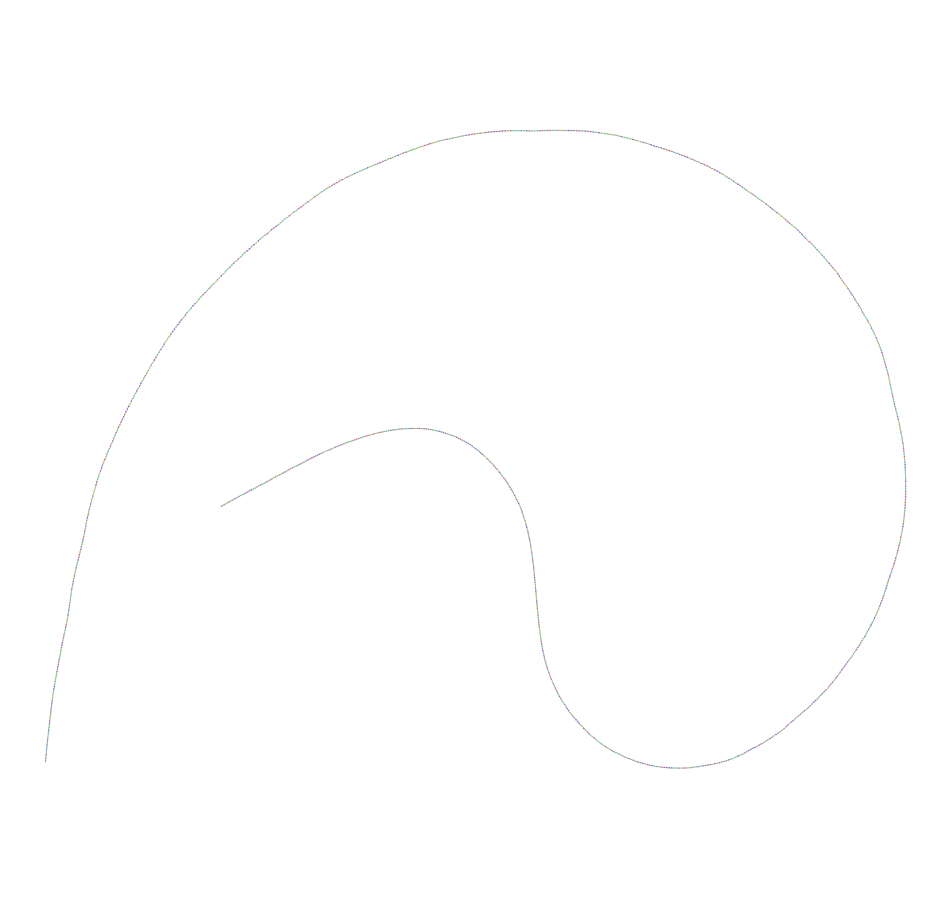
\includegraphics[width=0.5\textwidth]{../toy_dataset/r-k-45.png}
    \caption{Bandage visualization of DBG contigs for $k=45$ on reads\_r.fastq}
    \label{fig:dbg_k_45}
\end{figure} 

\begin{table}[h!]
\begin{center}
\begin{tabular}{ |c|c|c| }
    \hline
    Metric & k=35 & k=45 \\
    \hline
    sequence length & 1020 & 1040 \\
    number of contigs & 1 & 1 \\
    GC content (\%) & 51.37 & 51.25 \\
    genome fraction (\%) & 100.000 & 100.000 \\
    duplication ratio & 0.981 & 1.000 \\
    largest contig & 1020 & 1040 \\
    N50 & 1020 & 1040 \\
    N90 & 1020 & 1040 \\
    L50 & 1 & 1 \\
    misassemblies & 0 & 0 \\
    mismatches per 100 kbp & 0.00 & 0.00 \\
    indels per 100 kbp & 98.04 & 0.00 \\
    \hline
\end{tabular}
\caption{QUAST evaluation for $k=35$ and $k=45$ against reference\_r.fasta}
\label{tab:quast_k35_k45}
\end{center}
\end{table}

Figures \ref{fig:dbg_k_35} and \ref{fig:dbg_k_45} show the DBG for $k=35$ and $k=45$ on reads\_r.fastq visualized using Bandage. The DBG for $k=35$ has a bubble in the middle, which suggests that the assembly is not optimal to reconstruct the original genome. The DBG for $k=45$ has a more compact structure of a single contig, which suggests that the assembly is more optimal to reconstruct the original genome.
Table \ref{tab:quast_k35_k45} shows the QUAST evaluation for $k=35$ and $k=45$ against reference\_r.fasta. The DBG for $k=45$ has a perfect match to the reference genome, which can be seen in the genome fraction and duplication ratio. The DBG for $k=35$ has a lower duplication ratio and a sequence length but a perfect genome fraction, which suggest that the assembly is only missing a few nucleotides to completely match the reference genome.
The missed nucleotides are likely due to the bubble in the middle of the DBG for $k=35$.


\subsection{Task 1.3.3}

\subsubsection{ONT reads}
For DBG, I used $k = 40$. For OLC, I used $m = \text{min\_overlap} = 40$. These values had better assemblies than other values I tried (e.g. $k = 35,45$, etc. and $m = 30,50$, etc.).

Table \ref{tab:quast_mers} shows the QUAST evaluation for DBG and OLC on MERS virus data. The DBG has a better assembly than the OLC, which can be seen in the genome fraction and duplication ratio. The OLC has a higher duplication ratio and a lower genome fraction, which suggests that the implemented OLC algorithm is not as good at reconstructing the original genome.
Between the error-free and errored reads, both algorithms achieve obvious better performance in the error-free case bu having lower number of contigs and lower number of duplication ratios while having a high genome fraction. The OLC implementation is quite bad at reconstructing the original genome in both cases. In the errored reads case, OLC only reduced the number of contigs by 3. 
This is heavily influenced by the fact that the OLC \texttt{consensus} function is not optimized to solve the problem of reconstructing the original genome when having errors and small number of reads. I tried to implement a better \texttt{consensus} function, but it did not improve the performance of the OLC algorithm.


\begin{table}[h!]
\begin{center}
\begin{tabular}{ |c|c|c||c|c| }
    \hline
    Metric               & DBG (no-errors) & OLC (no-errors) & DBG (errors) & OLC (errors) \\
    \hline
    sequence length      & 29748  & 121258  & 76608 & 1505783 \\
    number of contigs    & 1      & 4       & 11 & 163 \\
    GC content (\%)      & 41.27  & 41.22    & 41.21 & 40.84 \\
    genome fraction (\%) & 98.765 & 96.670    & 98.738 & 98.655 \\
    duplication ratio    & 1.000  & 4.164    & 1.973 & 37.597 \\
    largest contig       & 29748  & 80399    & 17192 & 20439 \\
    N50                  & 29748  & 80399    & 12088 & 9201 \\
    N90                  & 29748  & 10145    & 1713 & 7834 \\
    L50                  & 1      & 1       & 3 & 73 \\
    misassemblies        & 0      & 29        & 0 & 0 \\
    mismatches per 100 kbp & 0.00 & 0.00     & 78.39 & 493.40 \\
    indels per 100 kbp   & 3.36   & 0.00     & 184.04 & 1463.10  \\
    \hline
\end{tabular}
\end{center}
\caption{QUAST evaluation for DBG and OLC on MERS virus data with ONT reads}
\label{tab:quast_mers}
\end{table}

In finding an optimal $m$ value for OLC, I tried different values of $m$ and found that $m = 3$ and $m = 2$ gave interesting results. Table \ref{tab:quast_mers_olc_m3_m2} shows the QUAST evaluation for OLC with $m = 3$ and $m = 2$ on MERS virus data.

They heavily reduce the number of contigs found while having high genome fractions. However, they both have high duplication ratios and high indels per 100 kbp, which suggests that they are not as good at reconstructing the original genome as DBG implementation.

Further work could be done to improve the OLC algorithm to reconstruct the original genome when having errors and small number of reads.

\begin{table}[h!]
\begin{center}
    \begin{tabular}{ |c|c|c| }
        \hline
        Metric               & m = 3 & m = 2 \\
        \hline
        sequence length      & 999925  & 537140   \\
        number of contigs    & 57      & 13        \\
        GC content (\%)      & 40.83  & 40.90    \\
        genome fraction (\%) & 97.600 & 94.767    \\
        duplication ratio    & 24.110  & 14.208    \\
        largest contig       & 73843  & 62932    \\
        N50                  & 19867  & 54062    \\
        N90                  & 8207  & 25366    \\
        L50                  & 13      & 5       \\
        misassemblies        & 36      & 34        \\
        mismatches per 100 kbp & 437.82 & 463.10     \\
        indels per 100 kbp   & 1359.61   & 1411.50     \\
        \hline
    \end{tabular}
    \end{center}
\caption{QUAST evaluation for OLC with $m = 3$ and $m = 2$ on MERS virus data}
\label{tab:quast_mers_olc_m3_m2}
\end{table}

\subsubsection{HiSeq reads}
Similar to the ONT reads, I used $k = 40$ for DBG and $m = \text{min\_overlap} = 40$ for OLC. Also, these values had better assemblies than other values I tried (e.g. $k = 35,45$, etc. and $m = 30,50$, etc.).

Table \ref{tab:quast_mers_dbg_olc} shows the QUAST evaluation for DBG and OLC on MERS virus data. In this case, both DBG and OLC have similar performance on the no-error case. However, OLC implementation fails horribly in the errored reads case.
This is also heavily due to the fact that the OLC \texttt{consensus} function is not optimized to solve the problem of reconstructing the original genome when having errors. I tried to implement a better \texttt{consensus} function, but it did not improve the performance of the OLC algorithm.

On the other hand, DBG implementation is able to reconstruct the original genome in the errored case relatively well with 94.425\% genome fraction and 1.014 duplication ratio. Also, relatively low number of contigs and indels per 100 kbp.

\begin{table}[h!]
\begin{center}
\begin{tabular}{ |c|c|c||c|c| }
    \hline
    Metric & DBG (no-errors) & OLC (no-errors) & DBG (errors) & OLC (errors) \\
    \hline
    sequence length        & 29553  & 29553  & 28835 & 18535 \\
    number of contigs      & 3      & 3      & 11 & 24 \\
    GC content (\%)        & 41.26  & 41.27  & 41.20 & 40.71 \\
    genome fraction (\%)   & 97.882 & 97.885 & 94.425 & 29.022 \\
    duplication ratio      & 1.002  & 1.002  & 1.014 & 1.157 \\
    largest contig         & 12290  & 12290  & 5155 & 2467 \\
    N50                    & 8725   & 8725   & 4682 & 734 \\
    N90                    & 8538   & 8538   & 1684 & 562 \\
    L50                    & 2      & 2      & 3 & 10 \\
    misassemblies          & 0      & 0 & 0  & 0 \\
    mismatches per 100 kbp & 0.00   & 0.00   & 38.16 & 692.11 \\
    indels per 100 kbp     & 10.15  & 0.00   & 38.16 & 266.96 \\
    \hline
\end{tabular}
\end{center}
\caption{QUAST evaluation for DBG and OLC on MERS virus data with HiSeq reads}
\label{tab:quast_mers_dbg_olc}
\end{table}

\subsection{Task 1.3.4}

Table \ref{tab:quast_mers_spades} shows the QUAST evaluation for SPAdes on MERS virus data. SPAdes is able to reconstruct the original genomes with high genome fractions and using only one contig assembly.

In the case of ONT reads, SPAdes and DBG have similar performance with similar genome fractions in the error-free and errored cases, but SPAdes has consistently lower duplication ratios and indels per 100 kbp, which can be understood as SPAdes only using one contig assembly.

In the case of HiSeq reads, SPAdes, DBG, and OLC have similar performance with similar genome fractions and GC content in the error-free case. However, in the errored case, SPAdes achieves better performance than DBG and OLC across all metrics.
This is expected as SPAdes has been developed and designed more rigorously while my implementations are simple and naive.

\begin{table}[h!]
\begin{center}
\begin{tabular}{ |c|c|c|c|c| }
    \hline
    Metric & ONT (no-errors) & ONT (errors) & HiSeq (no-errors) & HiSeq (errors) \\
    \hline
    sequence length & 29748 & 29751 & 29482 & 29482 \\
    number of contigs & 1 & 1 & 1 & 1 \\
    GC content (\%) & 41.27 & 41.25 & 41.26 & 41.26  \\
    genome fraction (\%) & 98.768 & 98.738 & 97.885  & 97.885 \\
    duplication ratio & 1.000 & 1.000 & 1.000 & 1.00 \\
    largest contig & 29748 & 29751 & 29482 & 29482 \\
    N50 & 29748 & 29751 & 29482 & 29482 \\
    N90 & 29748 & 29751 & 29482 & 29482 \\
    L50 & 1 & 1 & 1 & 1 \\
    misassemblies & 0 & 0 & 0 & 0 \\
    mismatches per 100 kbp & 0.00 & 0.00 & 0.00 & 0.00 \\
    indels per 100 kbp & 0.00 & 0.00 & 0.00 & 0.00 \\
    \hline
\end{tabular}
\end{center}
\caption{QUAST evaluation for SPAdes on MERS virus data}
\label{tab:quast_mers_spades}
\end{table}

\section{Task 2.1 Lizard Genome Assembly}

\section{Task 2.2 Assembly Evaluation}

\begin{thebibliography}{9}
\bibitem{olc_lecture_notes}
Langmead, B. (2024). Overlap-Layout-Consensus Assembly. Johns Hopkins University. 
\url{https://www.cs.jhu.edu/~langmea/resources/lecture_notes/assembly_olc.pdf}
\end{thebibliography}

\end{document}
